\section{Design}

\subsection{Tools and techniques}

\subsubsection{Tools}
\begin{itemize}
	\item \textbf{Github}: the source control platform used during the whole project development. Commit history, auto-generated progress statistics, progress tracking.
	\item \textbf{Visual Studio Code}: editor of choice, syntax highlighting, integrated debugger and unit test executor.
	\item \textbf{virtualenv}: Python environment isolation tool. Separates the development environment from the global machine environment, mitigates indirect permissions, dependencies and version incompatibility issues.
	\item \textbf{pip}: Python package installer. Keeps track of project dependencies, simplifies installation and deployment.
	\item \textbf{Lucidchart}: web-based tool for creation of UML diagrams and drawings. Used for planning and documentation purposes. 
	\item \textbf{pylint}: source-code bug and quality checker for Python following PEP8 style guide {18}. Highlights pure code practises and impose the use of good coding practices.
	\item \textbf{autoDocstring}: Visual Studio code extension for Python comment generation. Help to keep consistent commenting style and contributed to good coding practises.
	\item \textbf{Qt 5 Designer}: easy-to-use graphical user interface tool for designing and building Qt UI for the static part of the application.
\end{itemize}

\subsubsection{Libraries}
\begin{itemize}
	\item \textbf{pytest}: Python unit test framework. Extensively used during the whole prototype development process.
	\item \textbf{jsonpickle}: Third-party Python library used for exporting threat model as structured data.
	\item \textbf{ruamel.yaml}: Third-party Python library used for parsing yaml files. Yaml files were used to describe tools included in the tool set as well as providing 'caching' for the threat model entries. 
	\item \textbf{PyQt5}: a Python binding for a well known Qt v5 cross-platform C++ libraries set. It provides native look across common platforms and is used for the projects visual part. 
\end{itemize}

\subsubsection{Techniques}
\begin{itemize}
	\item \textbf{MVC pattern}
	
	Model-View-Controller architecture is used to separate the application data from it's visualization. Due to the inherited modularity of the project - combination of a threat model and a tool set - two separate instances of MVC pattern are used. 
	
	The first MVC instance is representing the threat model. The overall threat model data object is linked with the parent threat model Controller which contains the narrow purpose Controllers. Each Controller object in the parent Controller is linked to corresponding View object. View objects represent separate parts of threat model GUI. 
	
	The second MVC instance is needed to structure the tool set. There is generic object containing all the seprate penetration tool information. Each independent penetration tool has it's own Model representation. All penetration tools in the tool set have generated graphical user interfaces. These GUI's are created together with linked controllers by the tool Model objects in accordance to the tool data stored in those Models.
	
	\item \textbf{Facade pattern}
	
	Facade pattern is used to hide internal system complexity providing a simpler interface to use. In the project it is used to mask threat model internal relations providing a general "Threat Model" object to work with. The internal structure of a penetration tool object as well as the process of parsing it's configuration data is also encapsulated.
	
	\item \textbf{Interpreter pattern} (just defining language and parsing in recursively)
	
	Interpreter pattern is used while parsing penetration tool configuration files. Complete majority of pen testing tools can be run from the terminal. Unfortunately, various tool syntaxes tend to have fundamental differences. Therefore, one part of configuration parsing process is to interpret unique tool syntax which may also contain recursive patterns.
	
	\item \textbf{Observer pattern}
	
	Qt graphic components can make use of observer pattern to notify linked devices of different events. In Qt this pattern is called "Signal and Slot" mechanism. Signals can be "emitted" in response to system or custom actions and connected functions - Slots (can be enclosed in other objects) will execute in reply. It is used across the application to create dynamically linked and responsive GUI.
	
	\item \textbf{Object pooling}
	
	As the application uses threat pooling technique it supports parallel execution of multiple penetration testing tools. This way application main event loop is separated from individual tool execution.
	
	\item \textbf{Serialization}
	
	Serialization is used to preserve information kept in the threat model between work sessions. Threat modelling projects can be saved, closed and re-opened. Due to the way Python serializes objects the tool set implementation can be altered (e.g. a new version is released) still maintaining compatibility with threat model files created by older software versions.
	
\end{itemize}

\subsection{Application structure}

\subsubsection{High level design}
High level project structure is presented in figure \ref{fig:high-level-struct} below. \newline
It consists of two big and four smaller parts. The "Main" and "MainGui" components represent application parent classes. They are responsible for configuration, initialization and start up. During startup phase "ConfigManager" is called to load global system configurations such as interface folder location and cache configuration. The "InterfaceLoader" object is one of the central parts of the application. It's purpose, as the name suggests, is to parse penetration tool configuration files and create tool "Interface" instances. "Manager" object is supervises parallel penetration tool execution displays results.
"ThreatModel" object hides internal threat model complexity and loads it's display. "Completer" object is used to link threat model data with imported penetration tool options. It generates input suggestions during pen testing session. 
"MainGui" object loads initial parts of the application GUI structure and is responsible for threat model display.

Project layout diagram is provided in appendix \ref{sec:appendix-proj-struct}.

\begin{figure}[!htb]
	\center{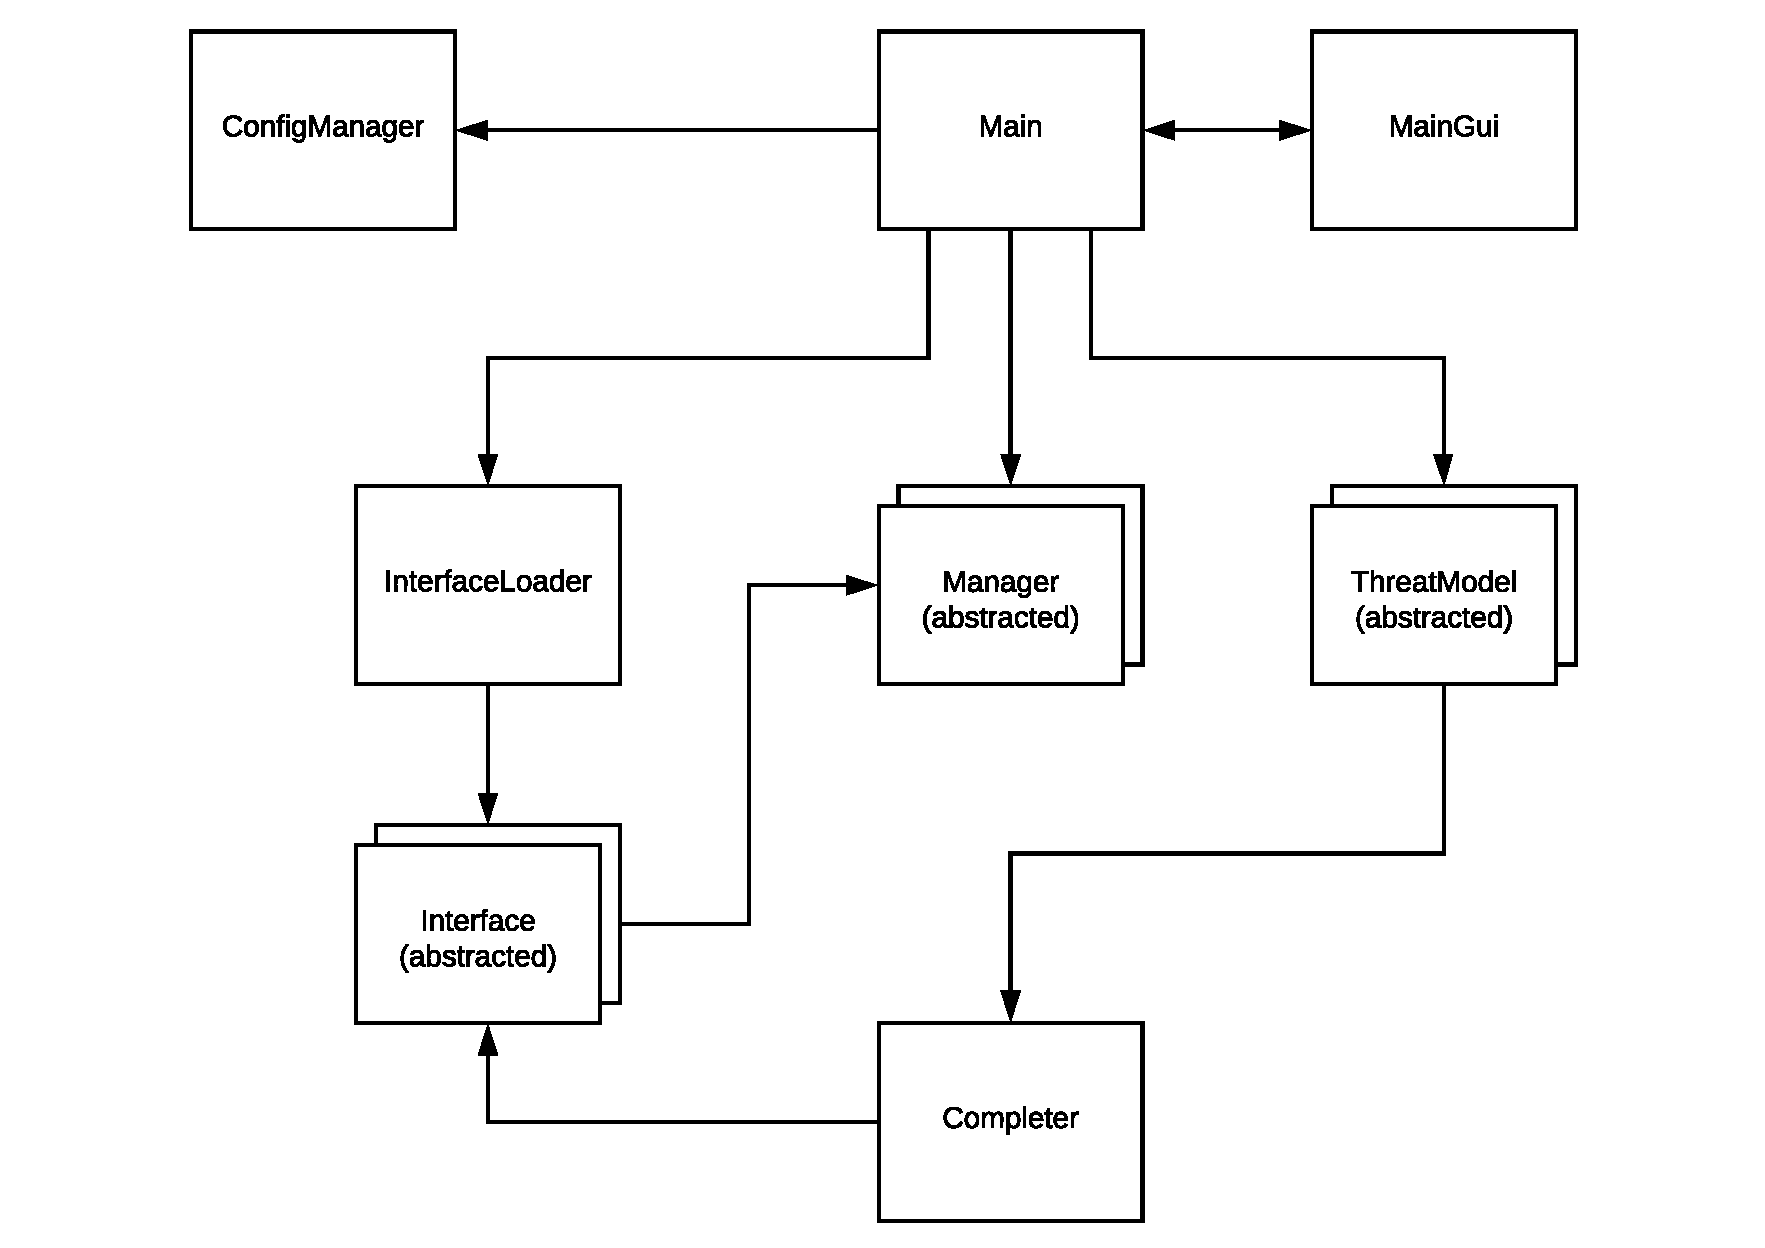
\includegraphics[width=\linewidth]
		{high_level_struct.pdf}}
	\caption{\label{fig:high-level-struct} High level project structure}
\end{figure}


\subsubsection{Penetration tool interface}
Simplified penetration tool interface structure is presented in figure \ref {fig:interface-struct} below. \newline
"InterfaceLoader" object is responsible of finding, parsing and storing discovered penetration testing tool interfaces. Individual penetration tools are described using configuration files. They define tools functionality and the way to map command line tool options to GUI entities. "Interface" objects are individual penetration tool representations in this project. "Interface" instances encapsulate overall penetration tool information required for it's use. Pen tool arguments are represented by the "Flag" and "Value" instances which are held in the "Instance" object. "FlagLabel" class is only used to group "Flag" instances and does not affect tools execution. 

Configuration file parsing is designed recursively, thus "InterfaceLoader" only does general configuration file structure checks. Similarly, "Interface" upon receiving data is only responsible for it's attributes, tool arguments are parsed by "Flag", "Value", "FlagLabel" and "Argument" classes respectively. Distributed parsing reduces complexity and splits up responsibilities making verification and testing easier.

Interface GUI is structured following MVC pattern and is generated automatically from parsed attributes. This design supports nested tool parameters without any additional configuration. Although, out of projects scope, Qt library provide a markup language similar to CSS. Therefore, due to the recursive nature of the GUI design, only insignificant modifications would be needed to provide a nicer user interface.

\begin{figure}[!htb]
	\center{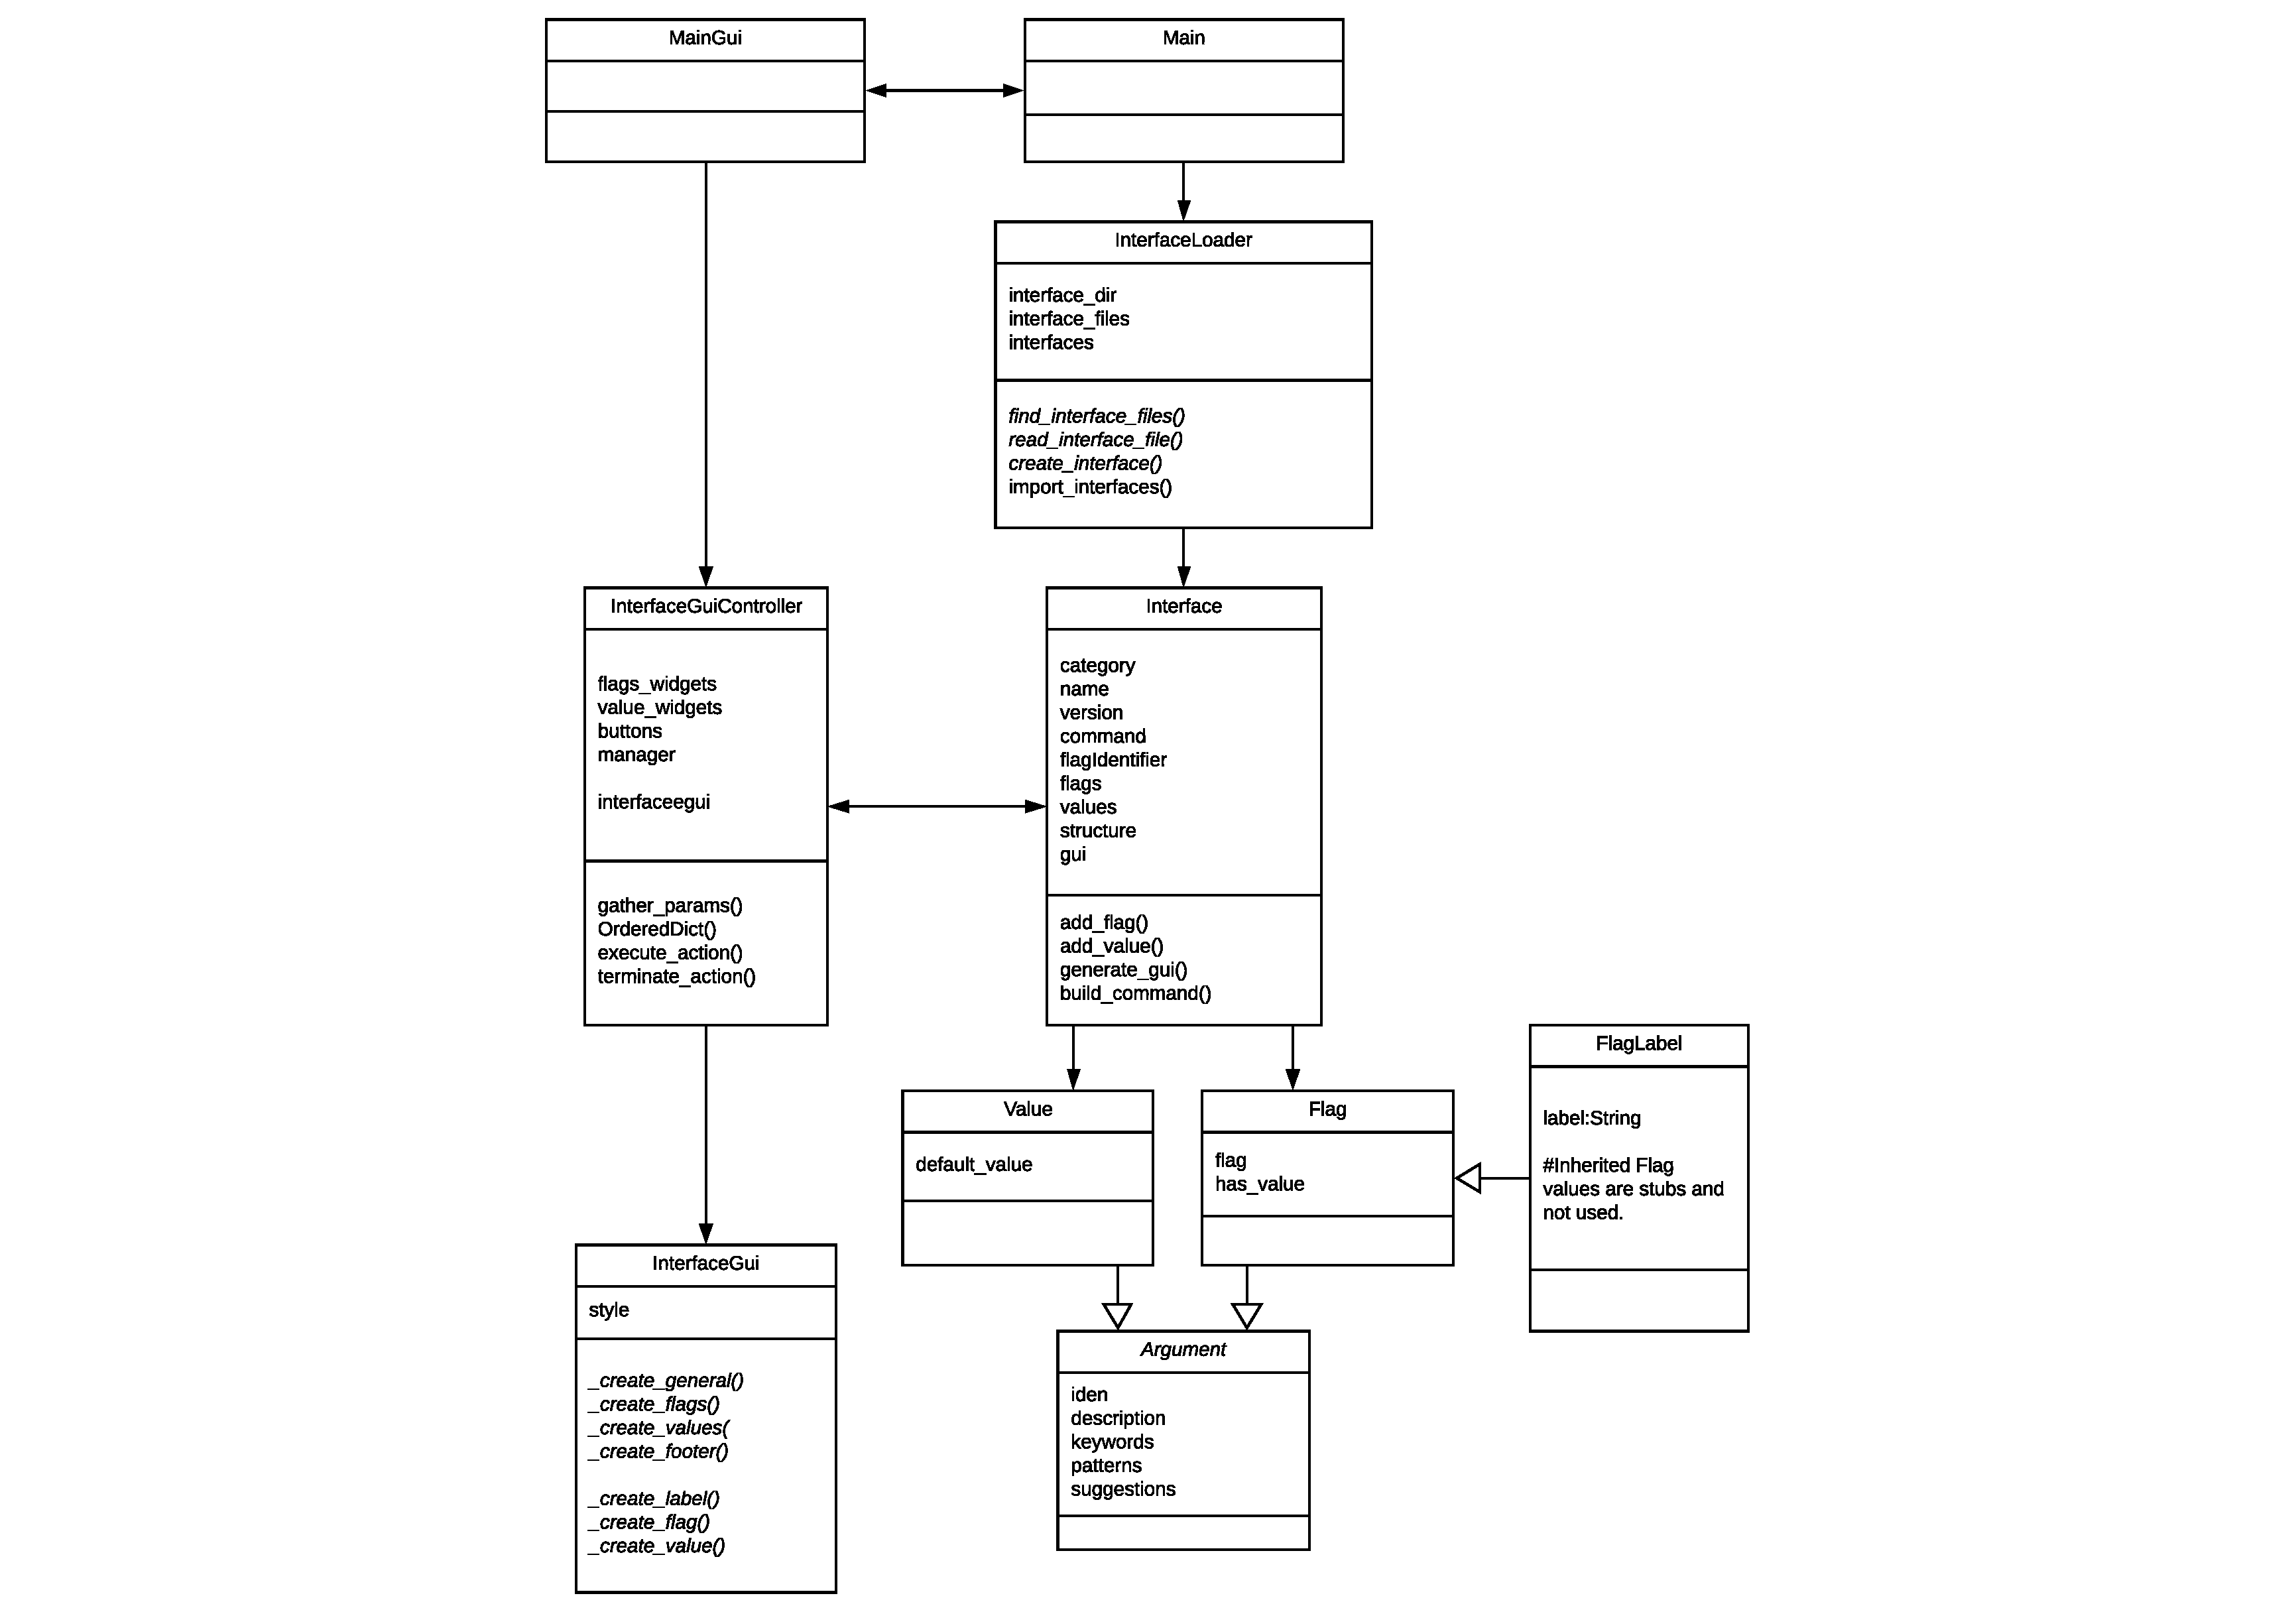
\includegraphics[width=\linewidth]
		{interface_diagram.pdf}}
	\caption{\label{fig:interface-struct} Simplified penetration tool interface related project part}
\end{figure}

\subsubsection{Tool execution and output}


\subsubsection{Threat model representation}
